\chapter{Performance Evaluation}\label{chap:performance}

Having validated the numerical implementations in the preceding chapter, 
we now present the performance analysis. This chapter addresses 
two of the central questions of this dissertation by quantifying 
the computational savings achieved by the MLMC method relative to the 
standard MC method and assessing the performance 
impact of different coupling strategies.

To this end, we outline the methodology used to measure 
performance. Following the approach detailed by Giles \cite{giles2015multilevel}
and used in the work by Cornalba 
and Fischer \cite{cornalba2025multilevel}, our primary metric for assessing 
theoretical performance is the normalised computational cost. For a range of 
target RMSEs, $\varepsilon$, we plot $\varepsilon^2 \times \mathrm{Cost}$
versus $\varepsilon$ on a log-log scale for both the MC and MLMC estimates. 
This metric is chosen because it 
connects directly to the MLMC Complexity Theorem. An optimal method 
with a theoretical complexity of $\mathcal{O}(\varepsilon^{-2})$ 
will appear as an approximately horizontal line.

$\mathrm{Cost}$ is determined using a semi-analytical estimate of the computational
work, derived from the number of samples $N_\ell$ used by the 
MLMC Algorithm, and a theoretical cost per sample, $C_\ell \propto 2^{\gamma \ell}$.
We have established that in all our implementations $\gamma = 3$.
We estimate the total MLMC Cost, $C_{\mathrm{MLMC}}$, for a given 
$\varepsilon$ therefore in the following way:

\begin{equation*}
    C_{\mathrm{MLMC}} := \sum_{\ell = 0}^L N_\ell C_\ell = \sum_{\ell = 0}^L N_\ell 2^{3\ell}.
\end{equation*}

For MC estimates, cost is calculated using the relationship between the
variance of the MC estimator and the number of samples taken, namely
$\varepsilon^2 \approx \frac{\mathbb{V}[P_\ell]}{N}$. We can infer 
from the MLMC Algorithm that the most refined level progressed to in order 
to achieve a given RMSE, $L$, 
is sufficient to reduce the discretisation error component of the RMSE, 
following Definition \ref{def:mse_rmse}. Therefore, we can quantify 
the MC Cost, $C_{\mathrm{MC}}$, as

\begin{equation*}
    C_{\mathrm{MC}} = N_{\mathrm{MC}} C_L = \frac{2 \mathbb{V}[P_L]}{\varepsilon^2}2^{3L}
\end{equation*}

where the factor of $2$ is included because in our MLMC Algorithm we 
require the statistical error of the estimator to be $\varepsilon / 2$.
We use our MLMC Algorithm implementation to obtain estimates of 
$\mathbb{V}[P_L]$.

We also include measured wall-clock timings, and present these in this chapter too.
The code used was written in C++20 \cite{cpp20standard}, 
and the timings were obtained running the implementation on Intel Gold 6538Y+ processors
\cite{intel_xeon_gold_6538y}.

\section{Stochastic Heat Equation - Performance Measurements}

Figure \ref{fig:performance_results_she} reports performance results for the three MLMC 
coupling strategies on the stochastic heat equation, for both QoIs.

\begin{figure}[htbp]
    \centering
    \begin{subfigure}{0.45\textwidth}
        \centering
        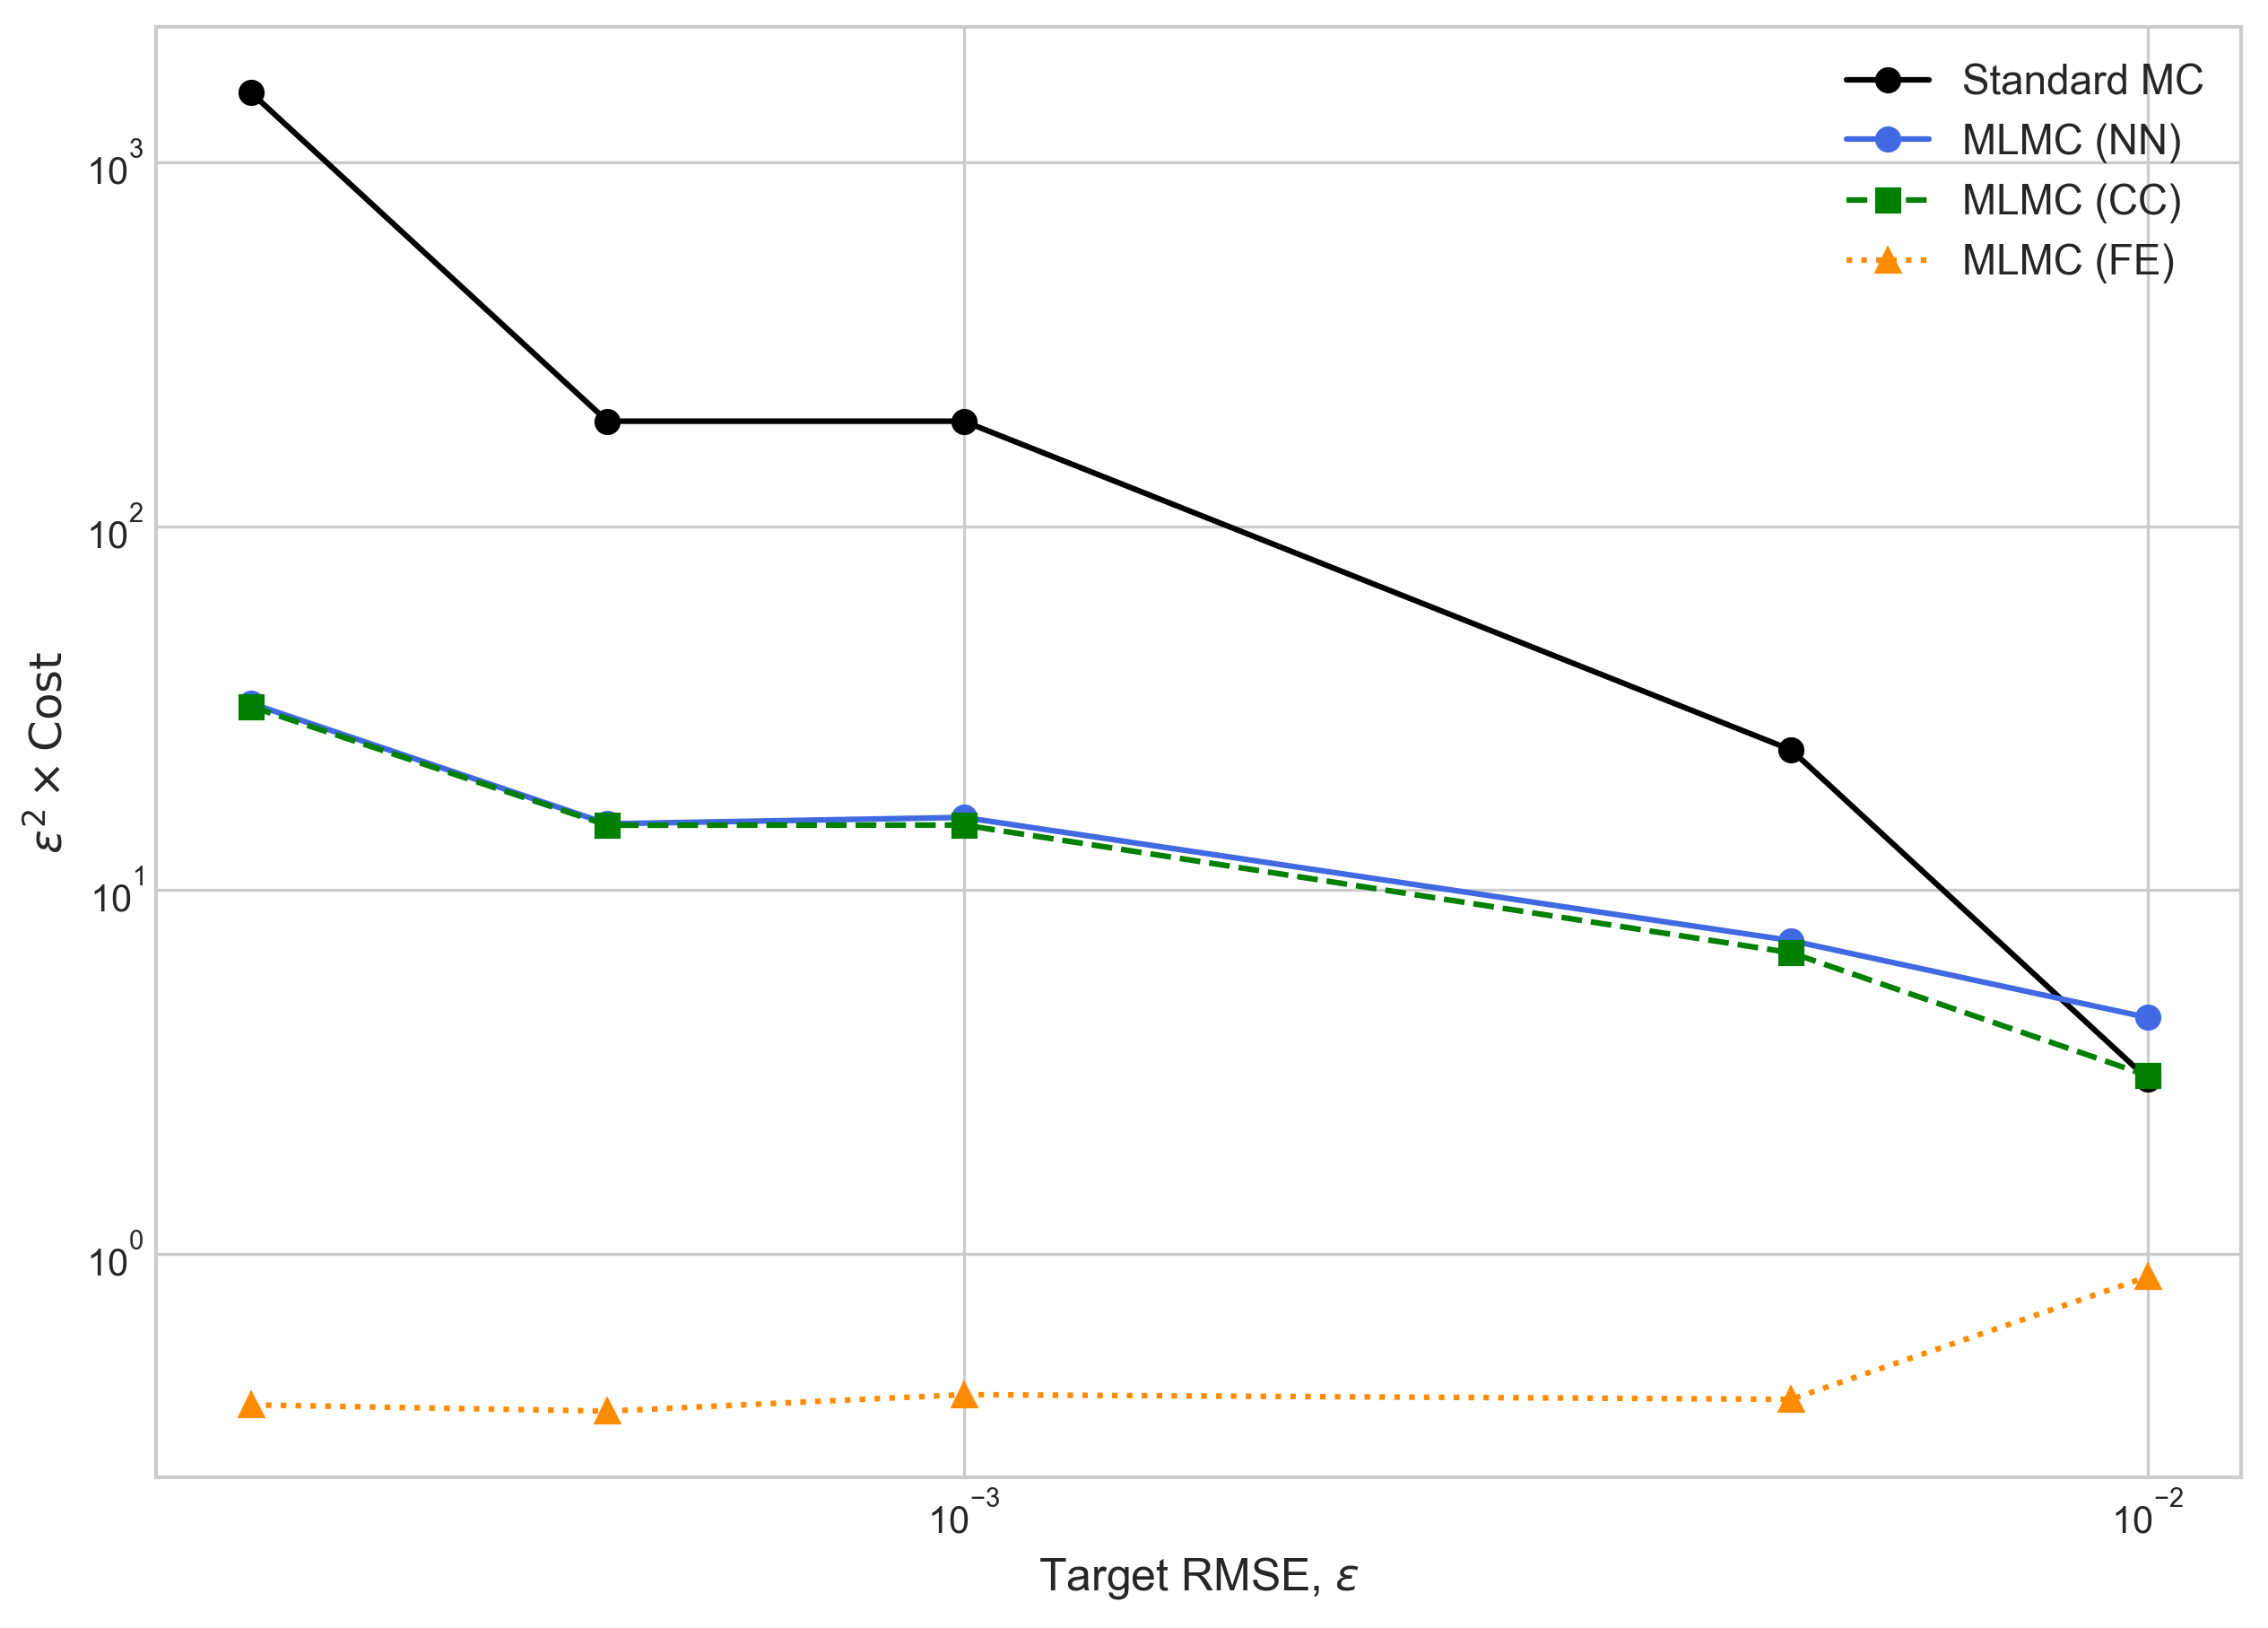
\includegraphics[width=\linewidth]{graphics/she_sq_amp_costs.png}
        \caption{Normalised cost vs target RMSE ($\varepsilon$) for Squared Amplitude.}
        \label{fig:she_sq_amp_performance}
    \end{subfigure}
    \hfill
    \begin{subfigure}{0.45\textwidth}
        \centering
        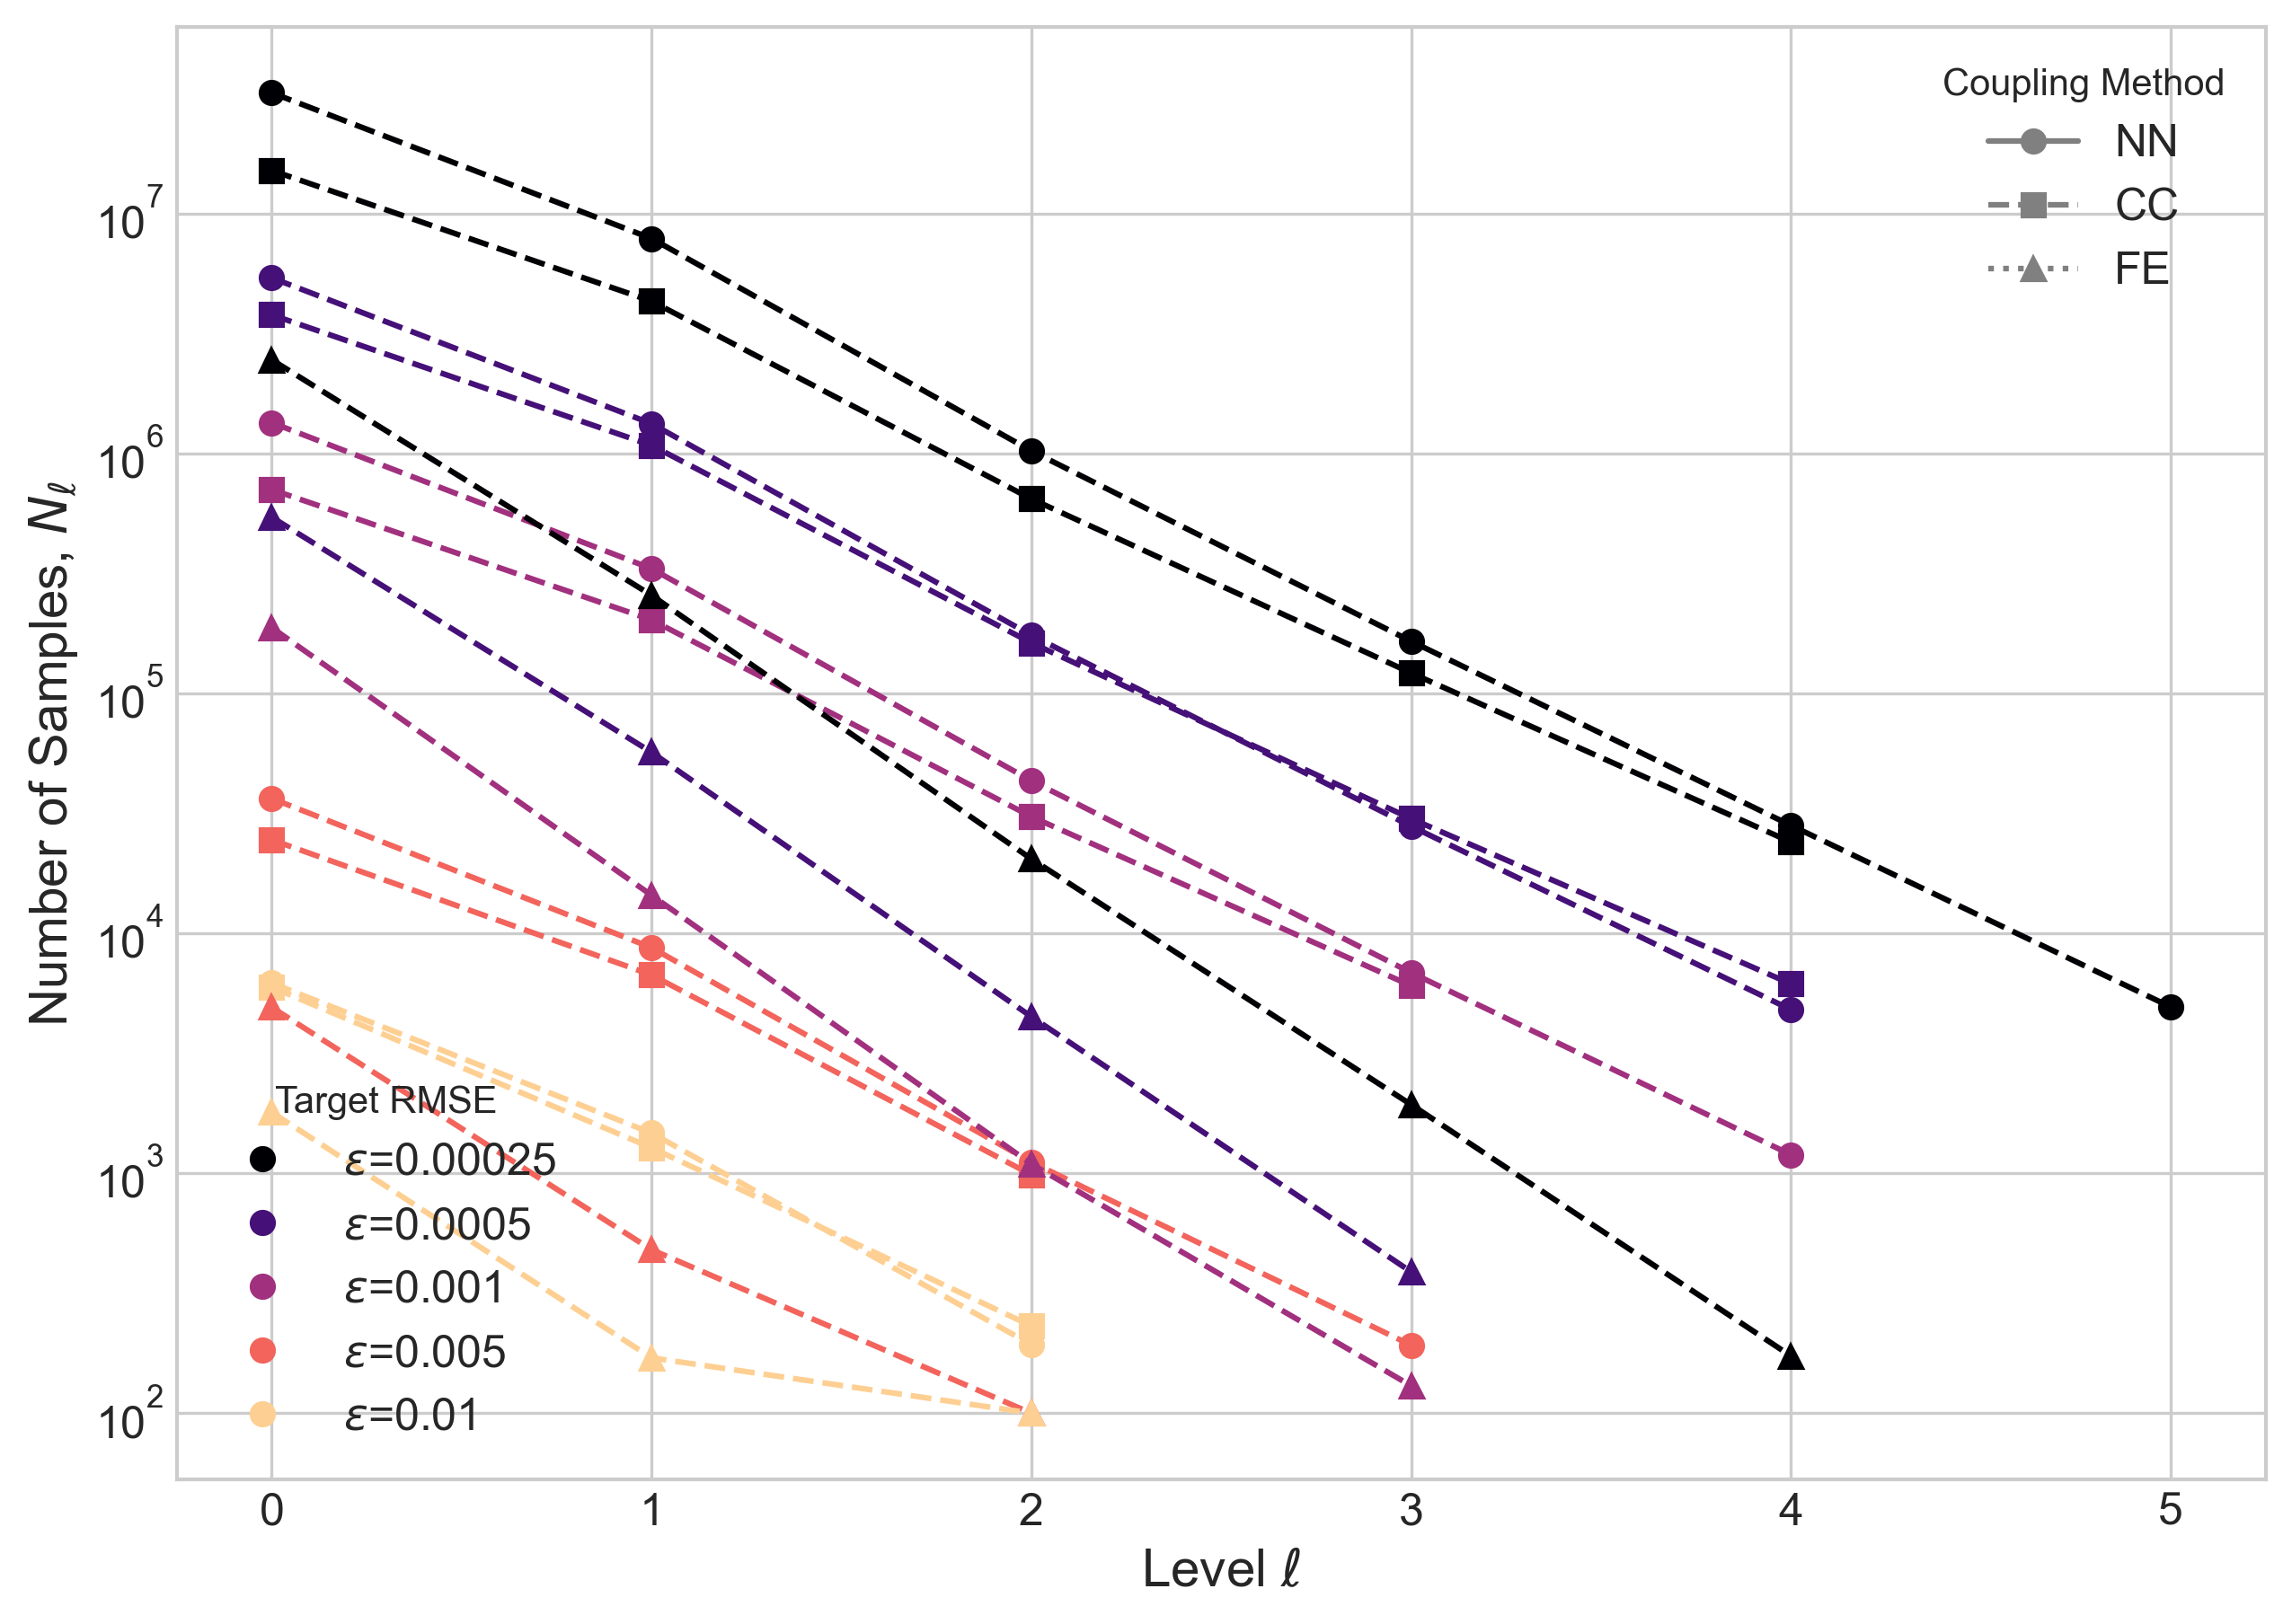
\includegraphics[width=\linewidth]{graphics/she_sq_amps_nums.png}
        \caption{Sample allocations for the Squared Amplitude.}
        \label{fig:she_sq_amp_levels_num}
    \end{subfigure}
    \begin{subfigure}{0.45\textwidth}
        \centering
        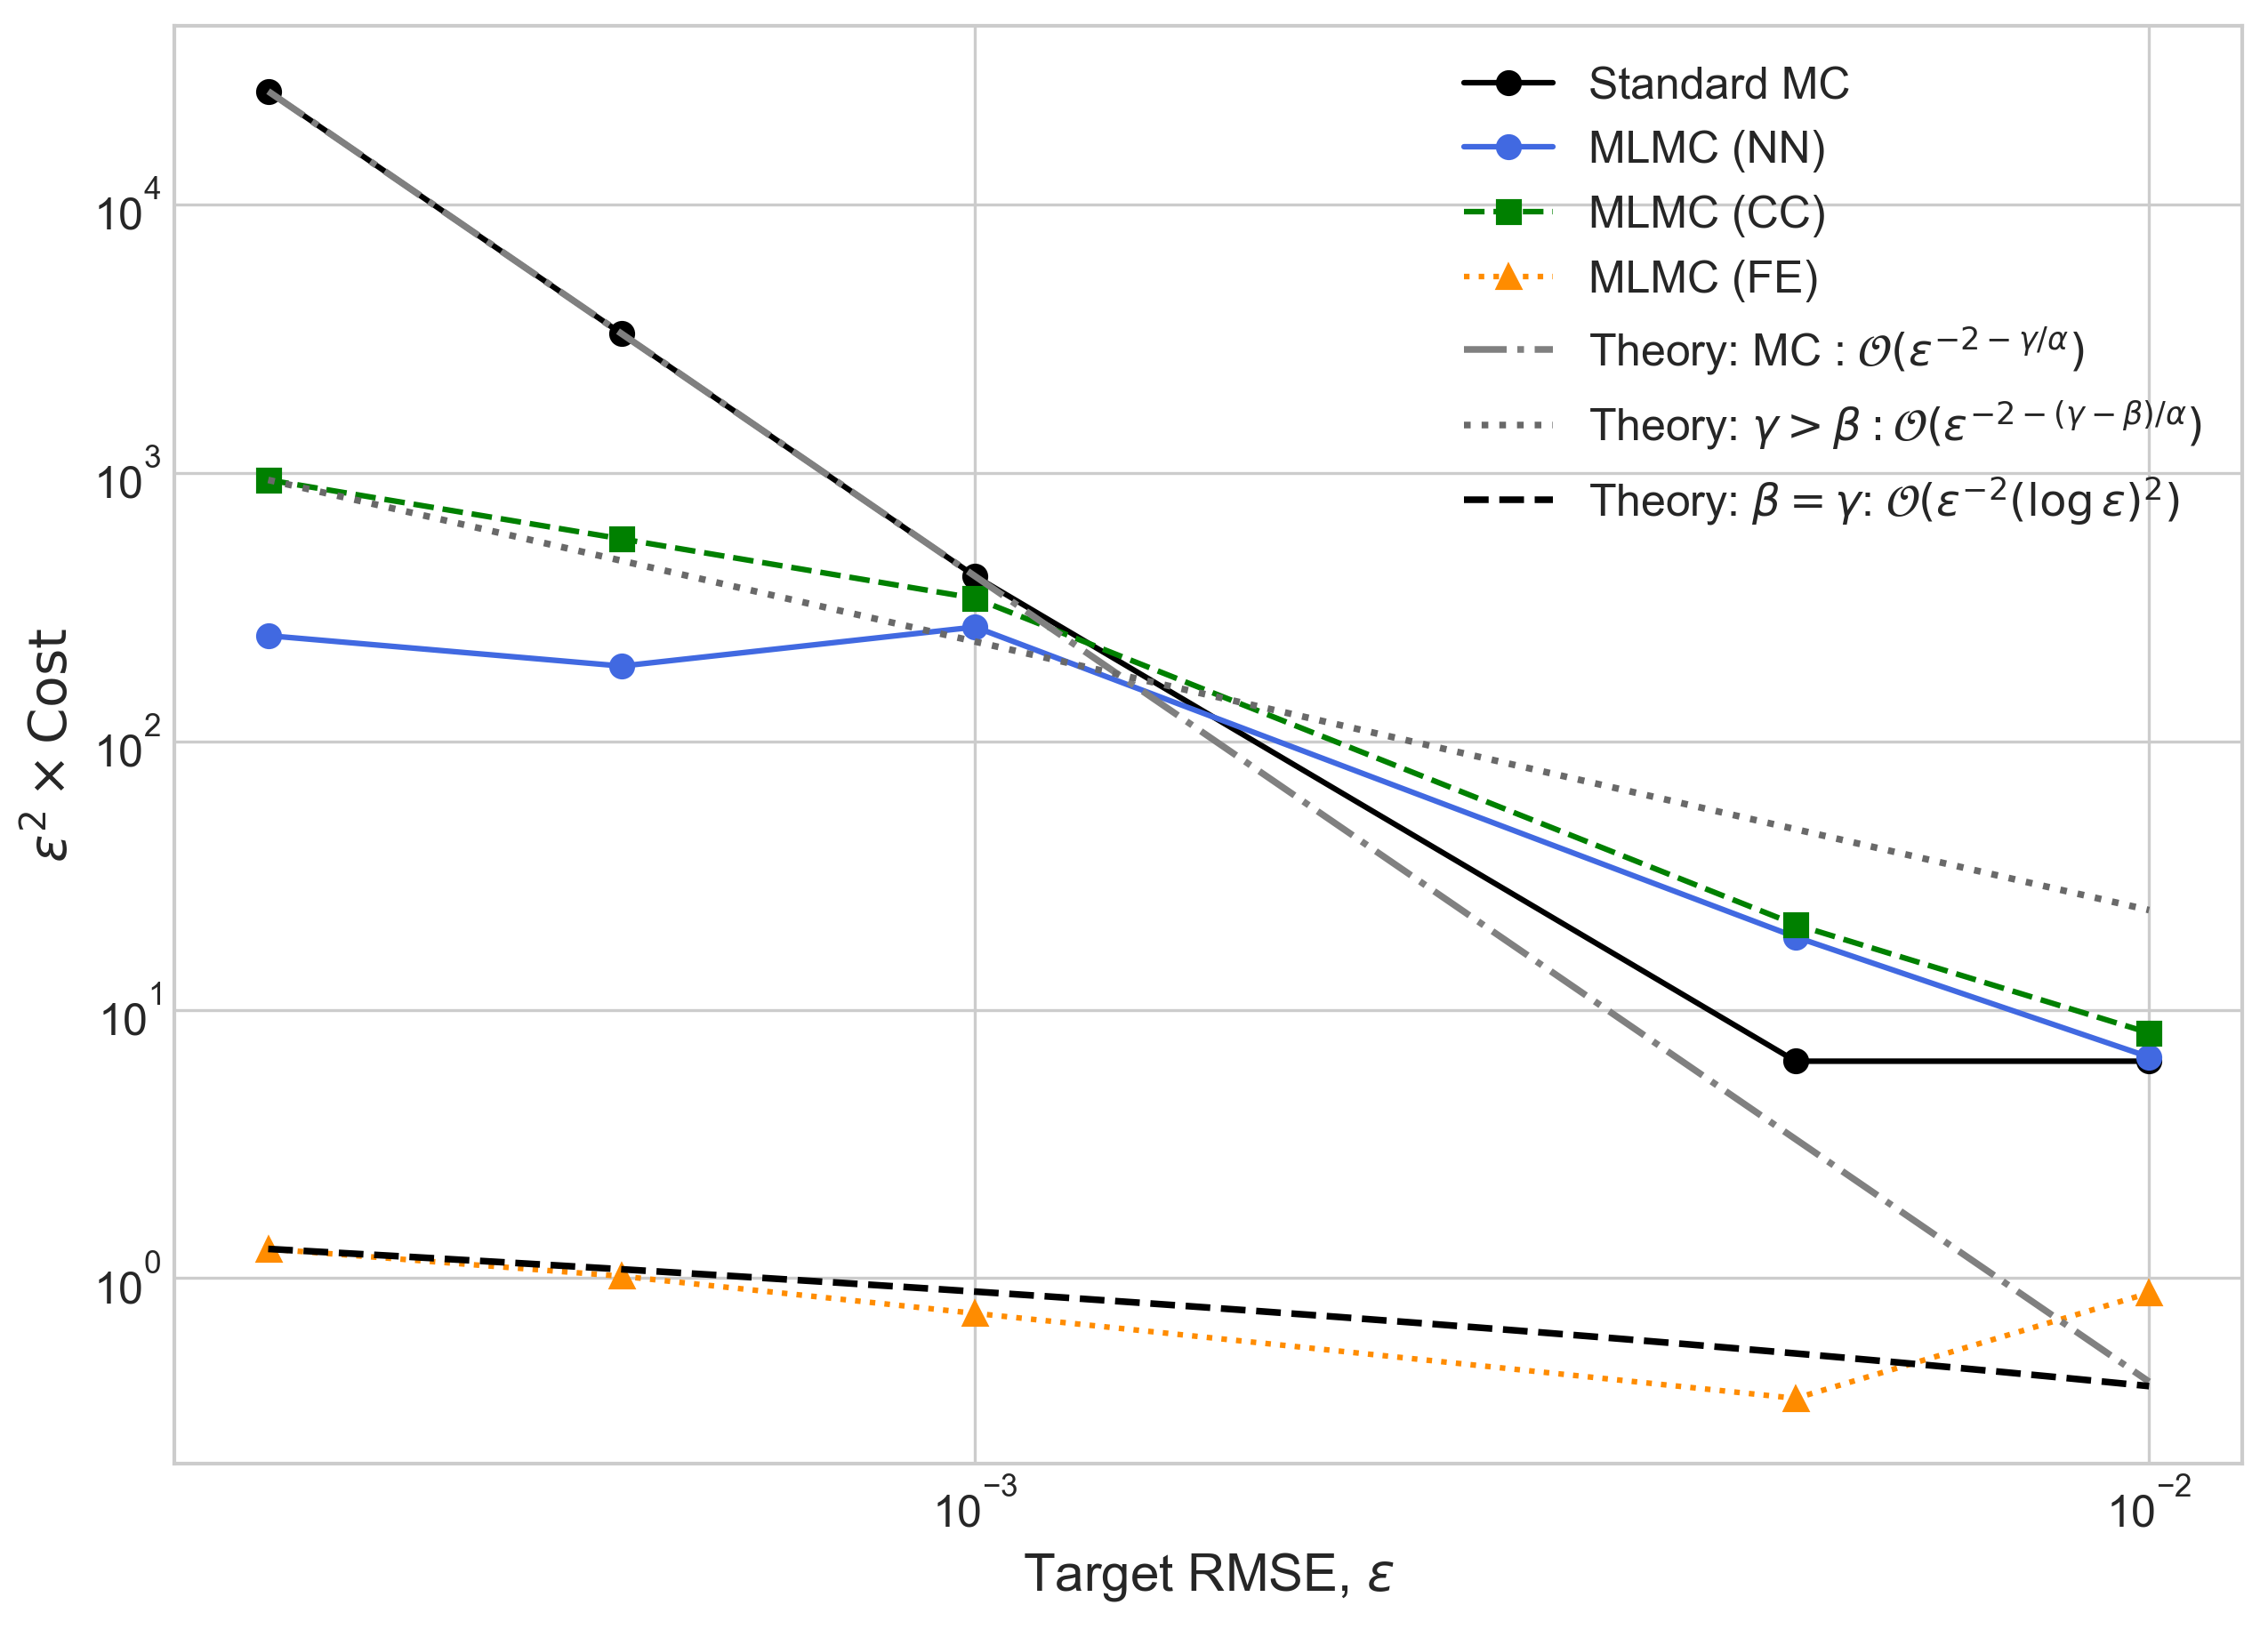
\includegraphics[width=\linewidth]{graphics/she_costs_energy.png}
        \caption{Normalised cost vs target RMSE ($\varepsilon$) for the System Energy QoI.}
        \label{fig:energy_performance}
    \end{subfigure}
    \hfill
    \begin{subfigure}{0.45\textwidth}
        \centering
        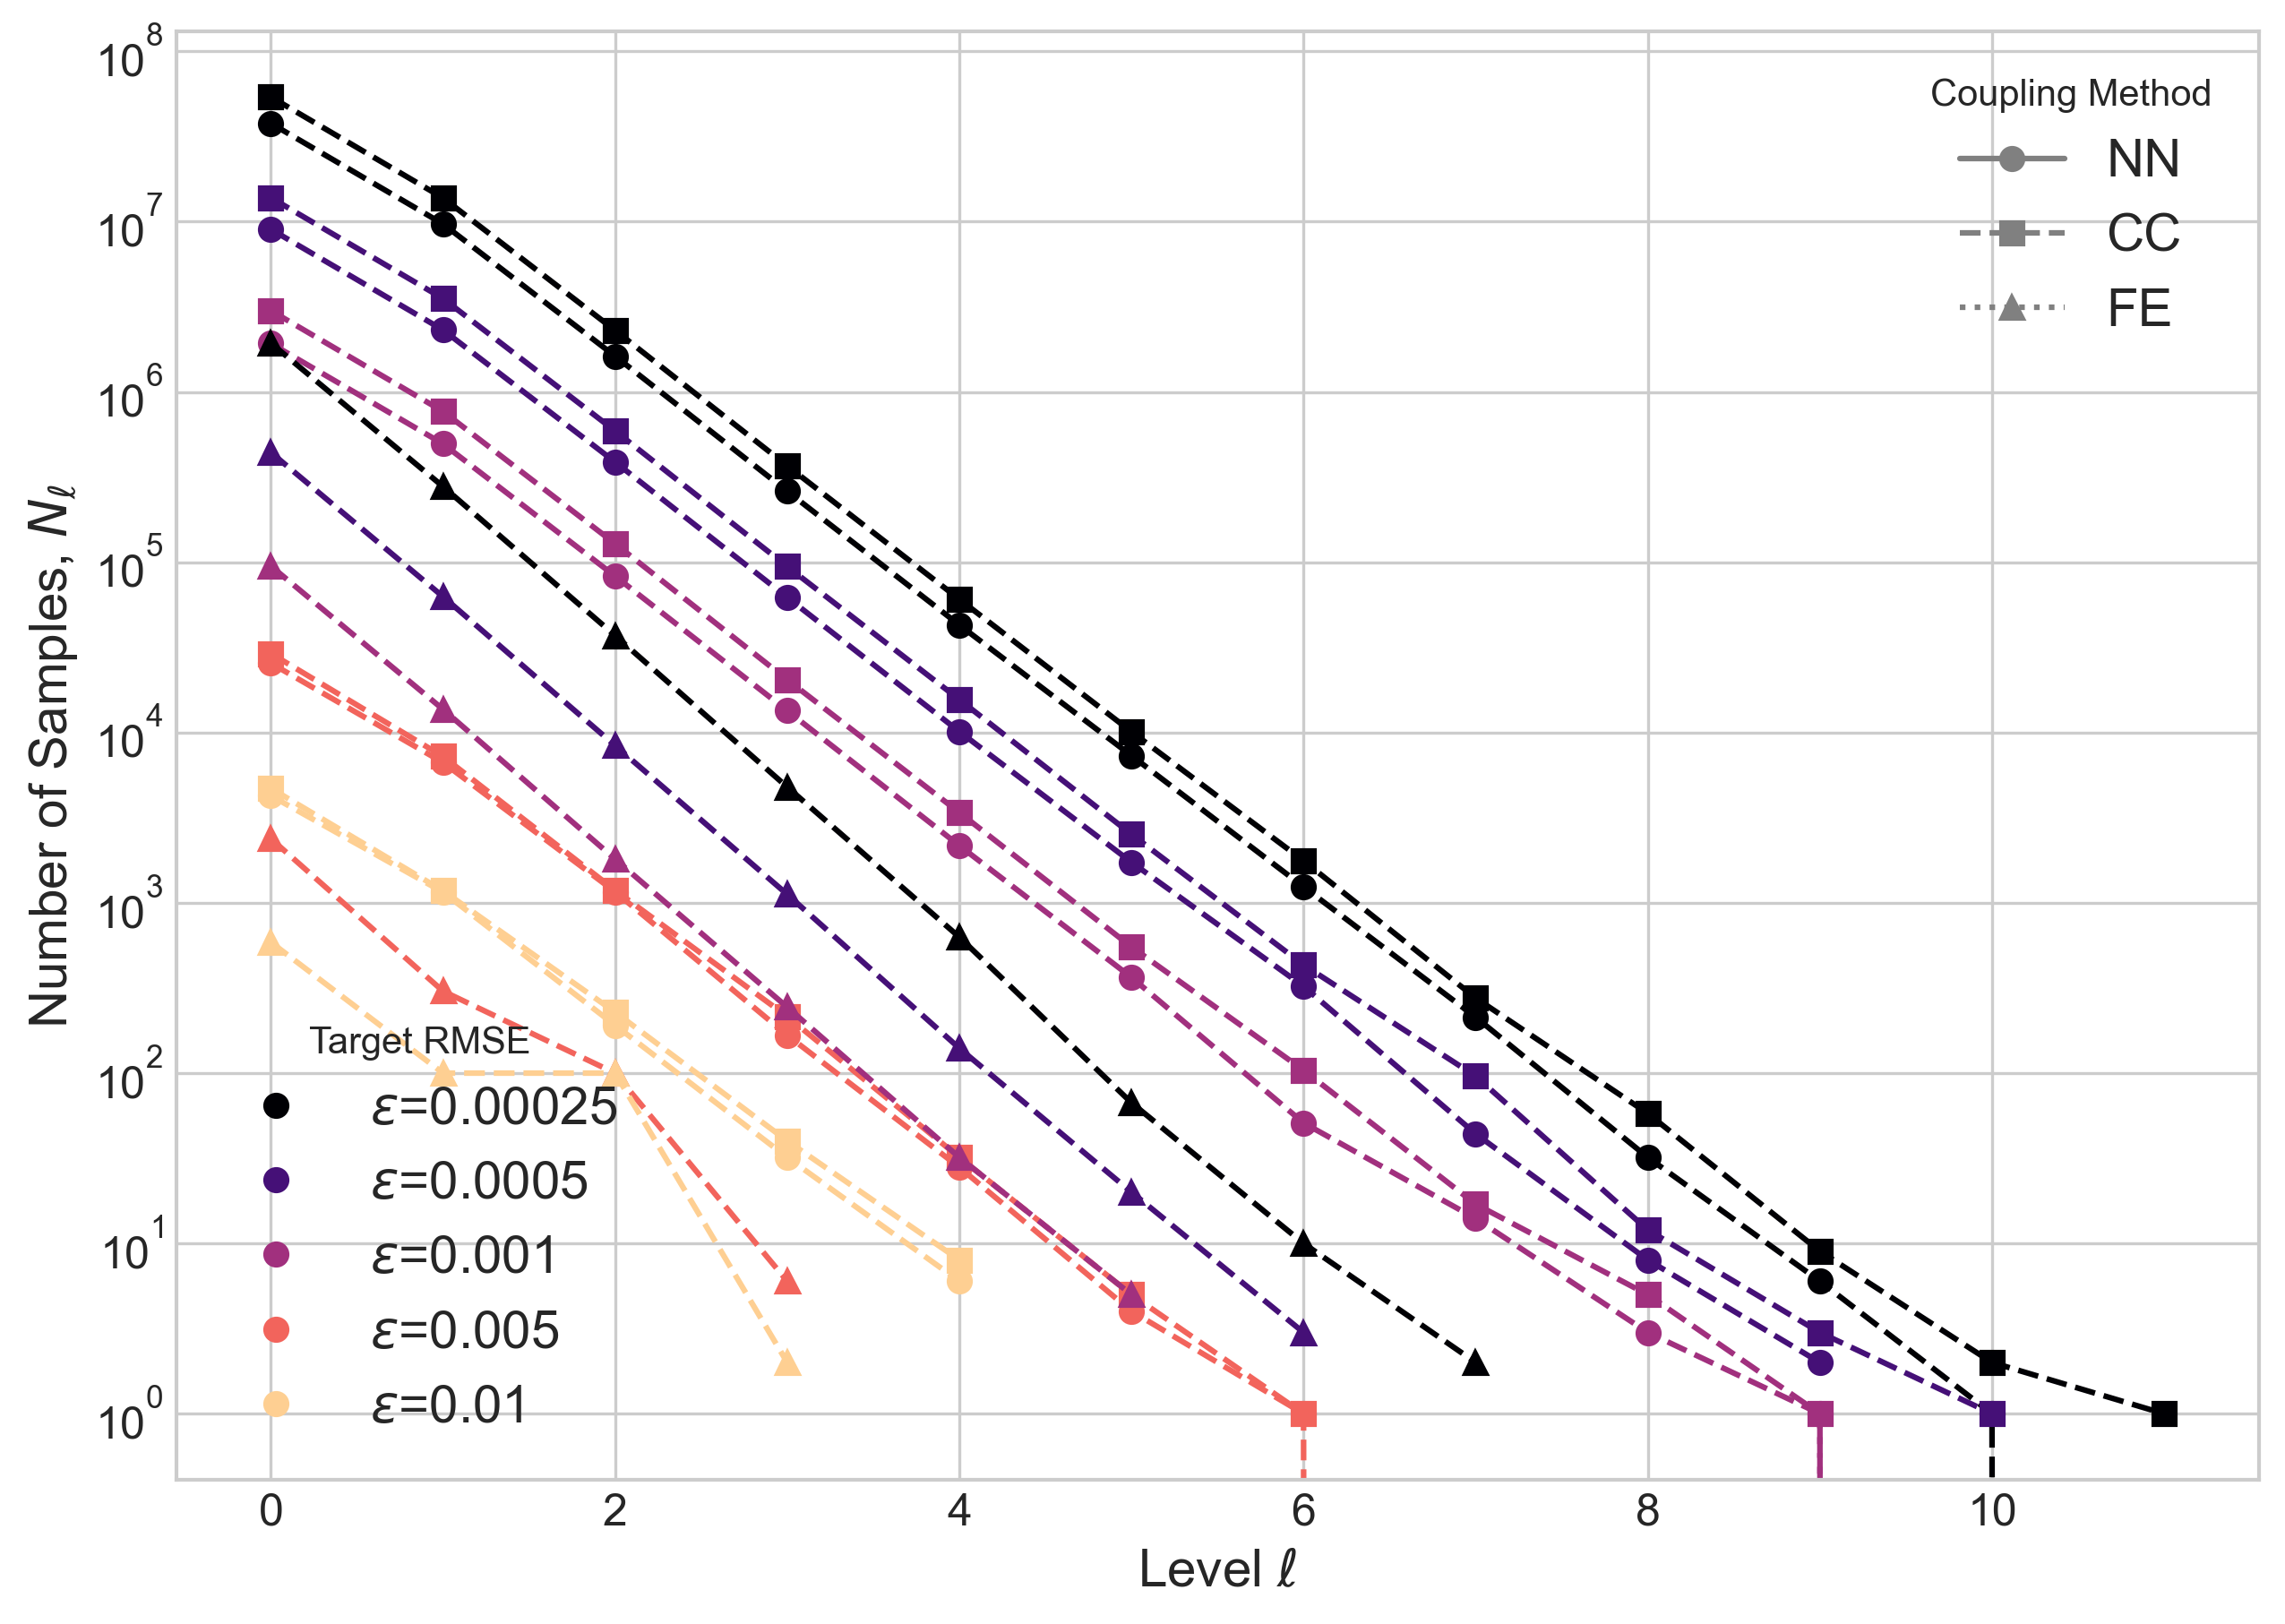
\includegraphics[width=\linewidth]{graphics/she_energy_nums.png}
        \caption{Sample allocations for the System Energy.}
        \label{fig:energy_levels_num}
    \end{subfigure}
    \caption{Performance results for the SHE. Top row shows results for the squared 
    amplitude for the first Fourier mode. The bottom row shows the results for the
    total system energy.}
    \label{fig:performance_results_she}
\end{figure}


\begin{table}[htbp]
    \centering
    \begin{tabular}{|l|c|c|r|}
        \hline
        \textbf{Coupling Method} & \textbf{Squared Amplitude} & \textbf{System Energy}\\
        \hline
        Nearest Neighbour & 0.4x-5.7x & 0.3x-106.6x \\
        Central Coupling & 0.8x-11.9x & 0.3x-28.0x \\
        Finite Element & 53.1-397.7x & 7.3x-20494.0x \\
        \hline
    \end{tabular}
    \caption{Smallest and largest cost scalings for different coupling mechanisms and QoIs.}
    \label{tab:she_cost_scalings}
\end{table}

Across both QoIs, the FE coupling is decisively superior, while NN and CC are broadly comparable. 
This is consistent with the decay rates we observed in Section 
\ref{sec:stoch_heat_validation}. In Figure 
\ref{fig:she_sq_amp_performance} we observe the optimal 
$\mathcal{O}(\varepsilon^{-2})$ scaling, which appears as a straight line on our plots. For 
the energy QoI, we observe the sub-optimal $\mathcal{O}(\varepsilon^{-2}\log^2(\varepsilon))$,
with cost only very slowly rising. This illustrates the benefits of 
faster variance decay.

Figures \ref{fig:she_sq_amp_levels_num} and \ref{fig:energy_levels_num}
demonstrate the tangible results of the faster variance decay, with significantly
fewer samples requiredbeing generated to achieve the target accuracy compared to the number 
required by the NN and CC methods.

In contrast, the NN and CC methods are effectively indistinguishable
in both cost and allocations.
Their cost plots show a clear downward slope, which is 
characteristic of the suboptimal case where $\beta < \gamma$. As RMSE decreases, 
we begin to observe significant cost reductions.
At larger RMSEs, we the NN and CC methods can result in 
the MLMC estimator being less efficient then the MC estimator. 
This is attributable to the variance reduction not 
scaling sufficiently when only a tiny number of samples/levels 
would suffice for MC.

The speed-up factors in Table 
\ref{tab:she_cost_scalings} show, even the suboptimal methods can provide 
a very significant computational savings over the standard Monte 
Carlo method, particularly when high accuracy is required. The FE method 
provides an extremely significant improvement over this.

\section{Dean-Kawasaki - Performance Measurements}

We now present the performance analysis for the Dean-Kawasaki equation. The results compare 
the efficiency of the standard Monte Carlo method against our MLMC implementations using 
both the NN and CC strategies. The key performance metrics are displayed in 
Figure \ref{fig:performance_results_dk}, with the overall speed-up factors 
summarised in Table \ref{tab:dk_cost_scalings}.


\begin{figure}[htbp]
    \centering
    \begin{subfigure}{0.45\textwidth}
        \centering
        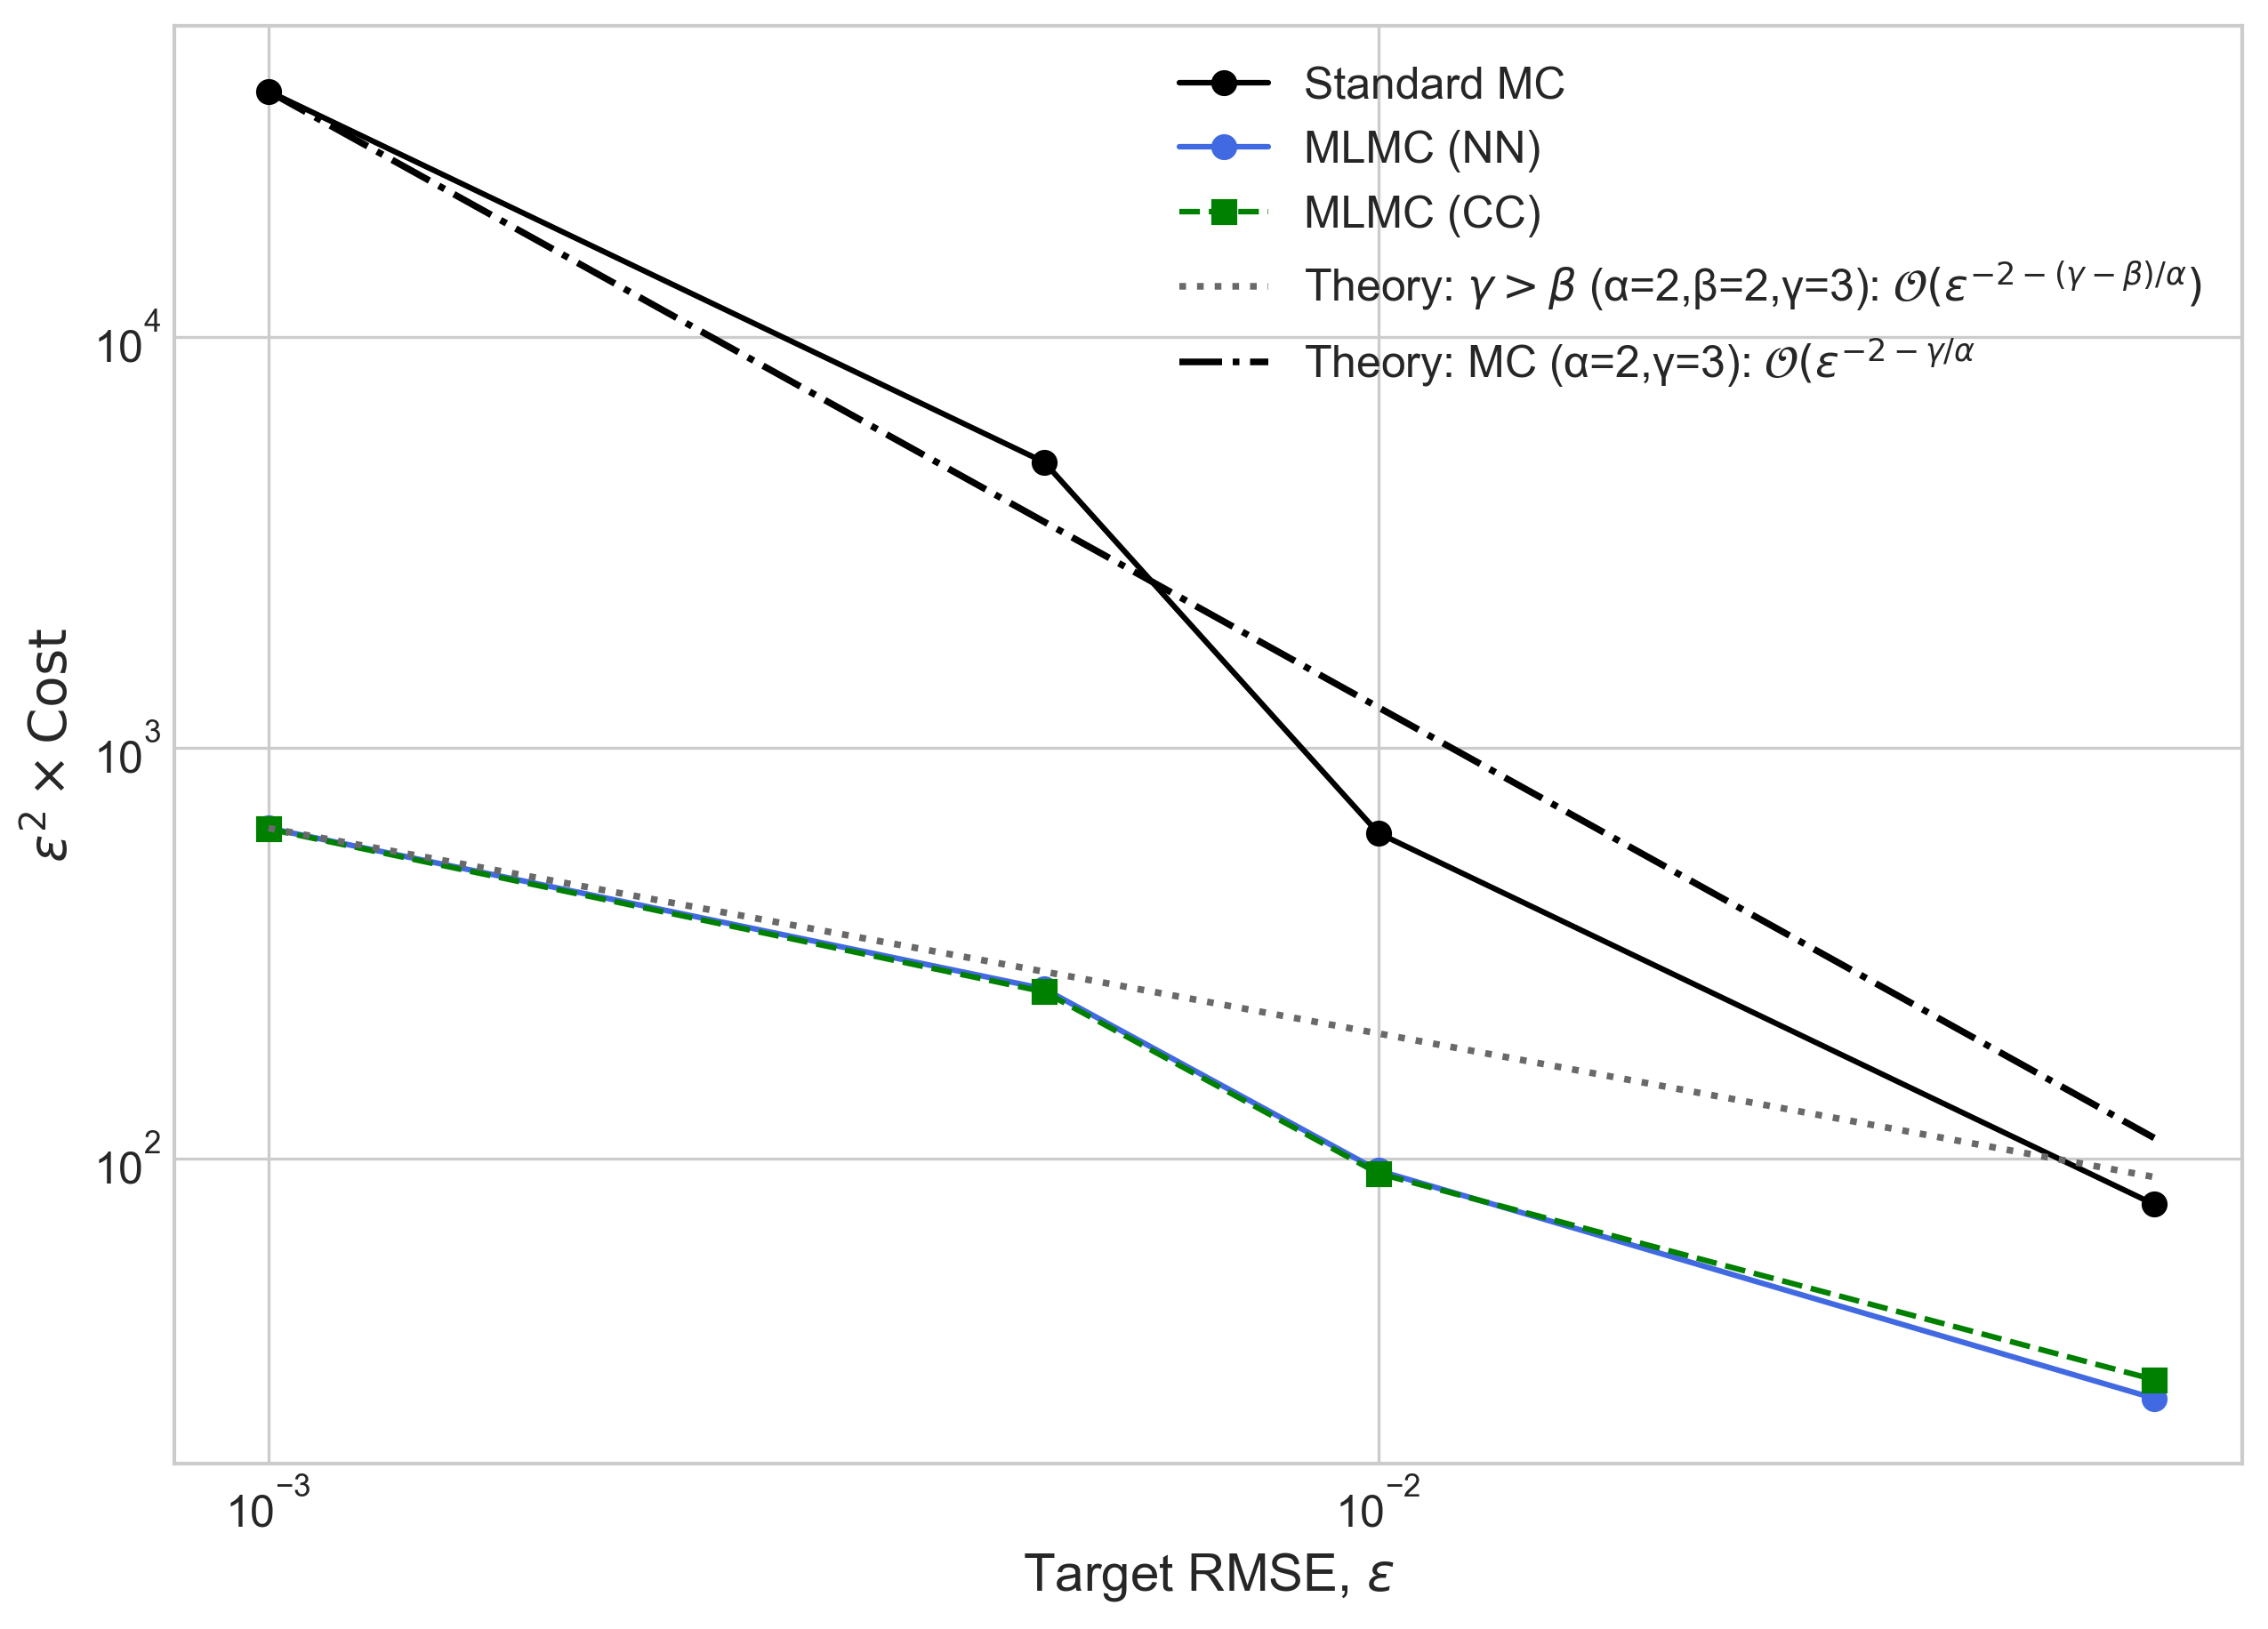
\includegraphics[width=\linewidth]{graphics/dk_costs.png}
        \caption{Normalised cost vs. target RMSE ($\varepsilon$).}
        \label{fig:dk_performance}
    \end{subfigure}
    \hfill
    \begin{subfigure}{0.45\textwidth}
        \centering
        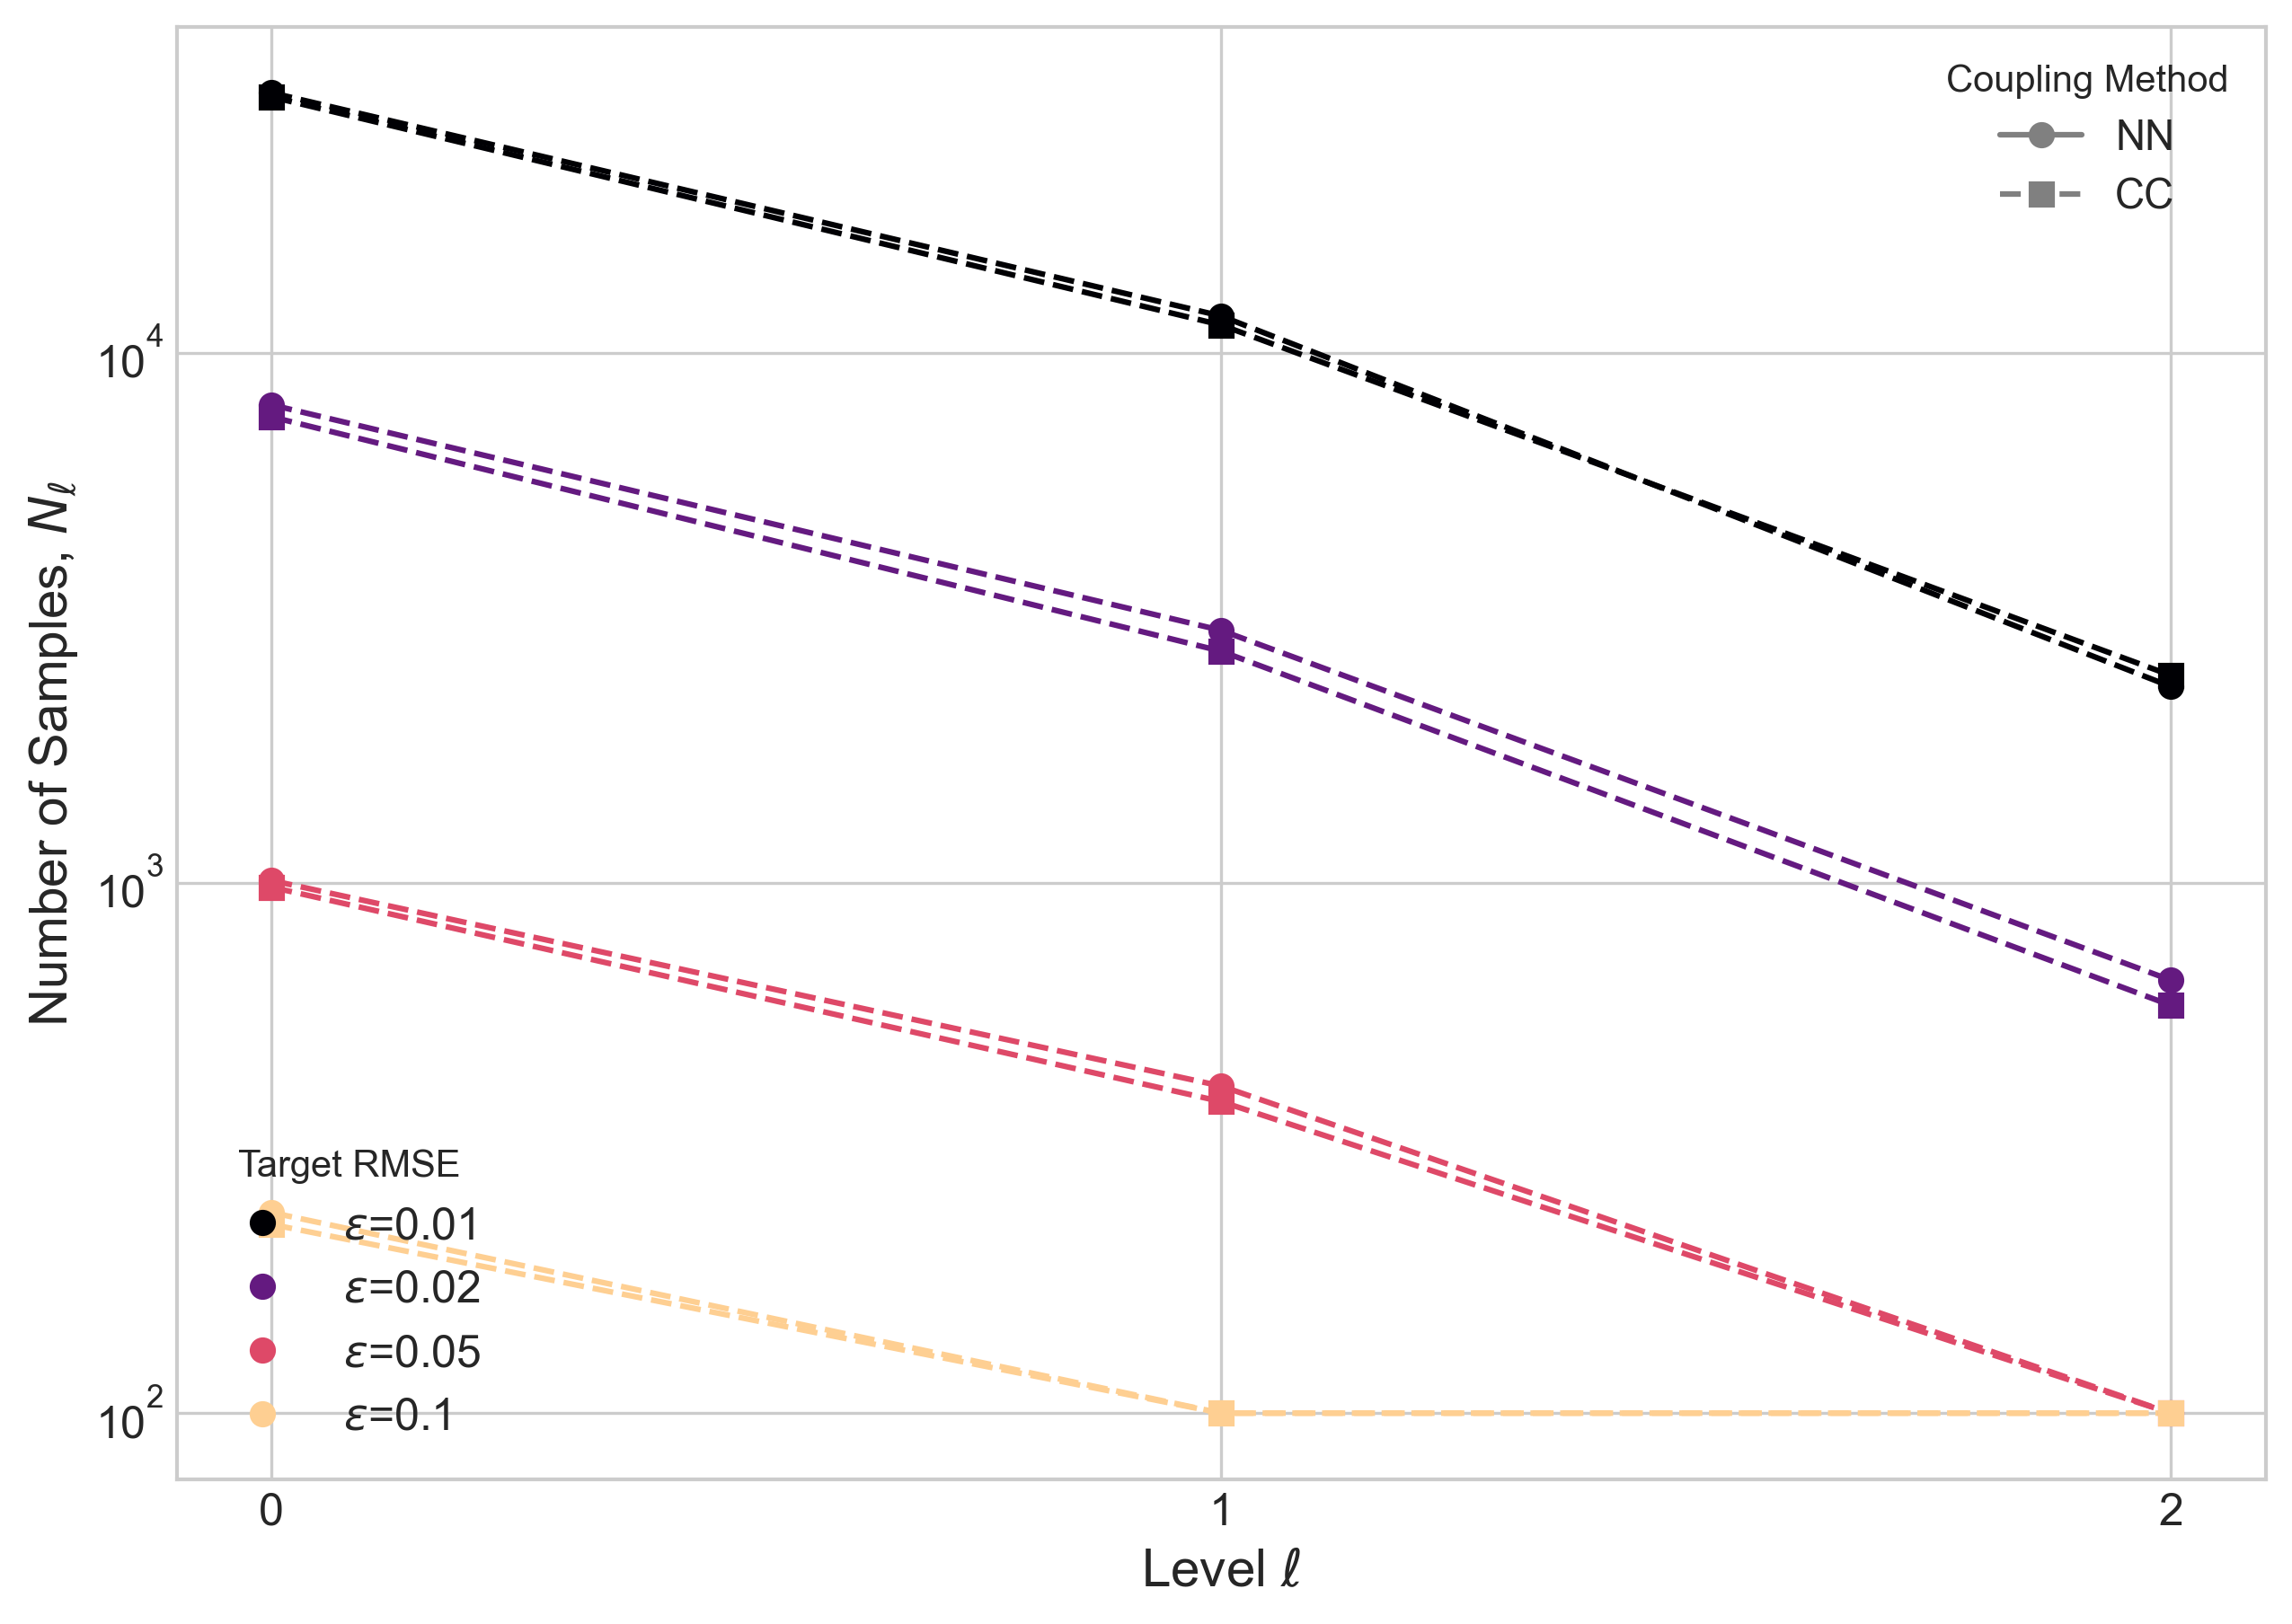
\includegraphics[width=\linewidth]{graphics/dk_nums.png}
        \caption{Sample allocation ($N_\ell$) vs level ($\ell$).}
        \label{fig:dk_num}
    \end{subfigure}
    \caption{Performance results for the MLMC implementation for the Dean-Kawasaki equation.}
    \label{fig:performance_results_dk}
\end{figure}


\begin{table}[htbp]
    \centering
    \begin{tabular}{|l|c|c|r|}
        \hline
        \textbf{Coupling Method} & \textbf{Mean Squared Fluctuations Speed-up Factor}\\
        \hline
        Nearest Neighbour & 3.0x-62.2x \\
        Central Coupling & 2.7x-62.5x \\
        \hline
    \end{tabular}
    \caption{Range of speed-up factors of MLMC over standard MC for the Dean-Kawasaki problem, for the 
    lowest and highest accuracies tested.}
    \label{tab:dk_cost_scalings}
\end{table}


The results clearly demonstrate that the MLMC method provides a significant 
computational advantage over the standard MC method for this problem. 
As shown in Figure \ref{fig:dk_performance}, the cost for both MLMC
implementations is substantially lower
than that of the standard MC estimator, aligning with the efficiency 
gains predicted by the MLMC theory.

We also observe that the Nearest Neighbour and Central Coupling strategies again 
exhibit 
identical performance. This is evident across all metrics. The normalised 
cost curves in Figure \ref{fig:dk_performance} are almost perfectly overlapping, 
the sample allocations in Figure \ref{fig:dk_num} are indistinguishable, 
and the final speed-up factors in Table \ref{tab:dk_cost_scalings} 
are the same. 

This result is consistent with the results from our validations, and demonstrate that 
neither method achieves a sufficient sample correlation similar to that achieved by the 
FE method. It was considered that the difference in symmetry, with the NN 
method discarding some noise and the CC method more symmetrically aligning obtaining 
some performance gains due to improved correlation between samples, but this 
does not appear to have any tangible impact on the efficiency for this problem.
